\chapter{Tensor-RNN: bridge between tensor networks and neural networks}
\label{ch:tensor-rnn}

~\cite{gao2017efficient}

\section{Vanilla MPS-RNN}

\begin{figure}[htb]
\centering
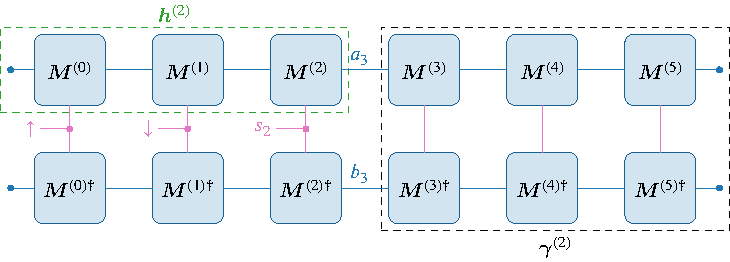
\includegraphics[width=0.8\linewidth]{ch9/mps_cond_prob.pdf}
\caption[Tensor diagram for conditional probability in MPS]{
This figure is reproduced from Fig.~S1 in the supplemental material of Ref.~\cite{wu2023tensor}.
}
\label{fig:mps-cond-prob}
\end{figure}

\begin{figure}[htb]
\centering
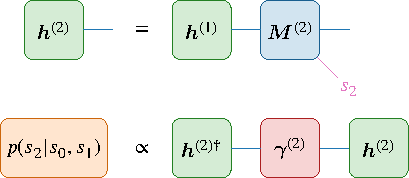
\includegraphics[width=0.5\linewidth]{ch9/mps_h_p.pdf}
\caption[Tensor diagram for memory update of vanilla MPS-RNN]{
This figure is reproduced from Fig.~1~(b) in Ref.~\cite{wu2023tensor}.
}
\label{fig:mps-h-p}
\end{figure}

\begin{figure}[htb]
\centering
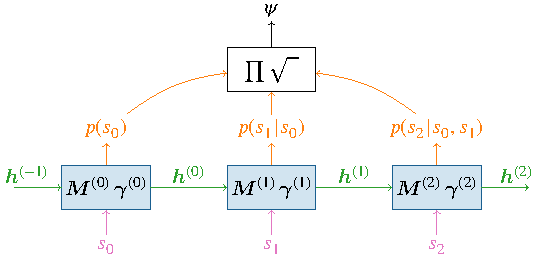
\includegraphics[width=0.7\linewidth]{ch9/rnn_psi.pdf}
\caption[Computational graph for vanilla MPS-RNN]{
This figure is reproduced from Fig.~1~(a) in Ref.~\cite{wu2023tensor}.
}
\label{fig:rnn-psi}
\end{figure}

\begin{figure}[htb]
\centering
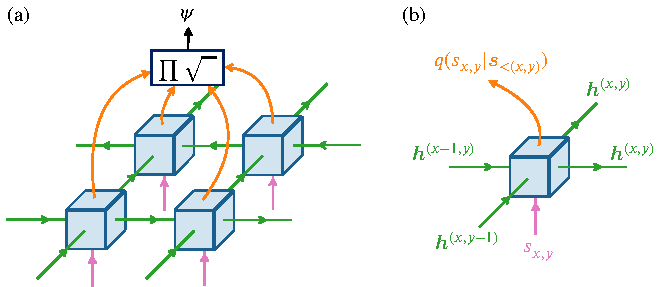
\includegraphics[width=0.8\linewidth]{ch9/tensor_rnn_all.pdf}
\caption[Computational graph for tensor-RNN]{
This figure is reproduced from Fig.~2 in Ref.~\cite{wu2023tensor}.
}
\label{fig:tensor-rnn-all}
\end{figure}

\begin{figure}[htb]
\centering
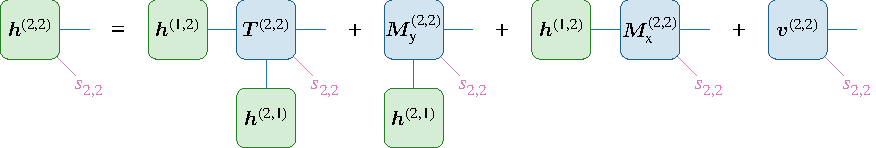
\includegraphics[width=\linewidth]{ch9/tensor_rnn_h.pdf}
\caption[Tensor diagram for memory update of tensor-RNN]{
This figure is reproduced from Fig.~3 in Ref.~\cite{wu2023tensor}.
}
\label{fig:tensor-rnn-h}
\end{figure}

\section{1D MPS-RNN}

\section{2D MPS-RNN and tensor-RNN}

Another architecture~\cite{hibat2021variational, hibat2022supplementing}

Mixture of neural and tensorial layers~\cite{chen2023antn}

Recurrent arithmetic circuits~\cite{levine2017long, levine2019quantum}

\section{Numerical results}

\begin{figure}[htb]
\centering
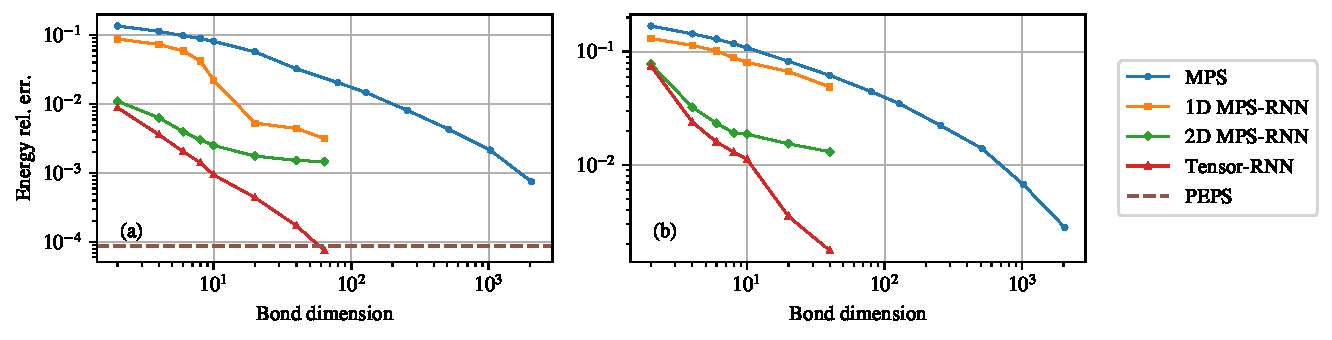
\includegraphics[width=1.05\linewidth]{ch9/tensor_rnn_energy_chi.pdf}
\caption[Variational energy vs. bond dimension for tensor-RNN]{
This figure is reproduced from Fig.~4 in Ref.~\cite{wu2023tensor}.
}
\label{fig:tensor-rnn-energy-chi}
\end{figure}

\begin{figure}[htb]
\centering
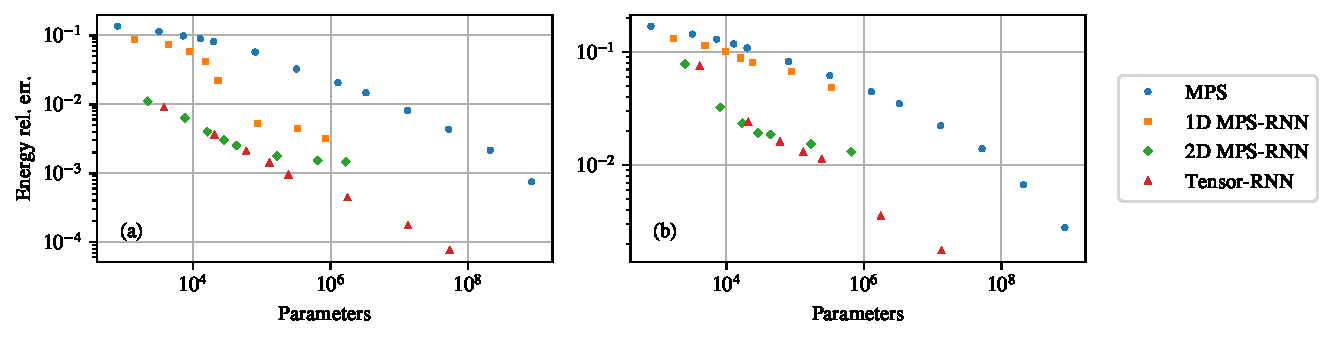
\includegraphics[width=1.05\linewidth]{ch9/tensor_rnn_energy_param.pdf}
\caption[Variational energy vs. number of parameters for tensor-RNN]{
This figure is reproduced from Fig.~S3 in the supplemental material of Ref.~\cite{wu2023tensor}.
}
\label{fig:tensor-rnn-energy-param}
\end{figure}

\begin{figure}[htb]
\centering
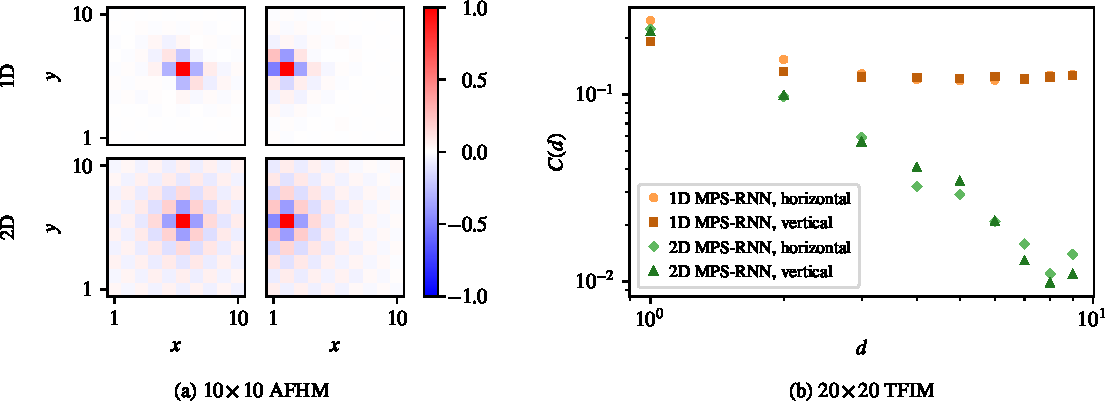
\includegraphics[width=\linewidth]{ch9/tensor_rnn_corr.pdf}
\caption[Spin correlations in MPS-RNN]{
This figure is reproduced from Fig.~S4 in the supplemental material of Ref.~\cite{wu2023tensor}.
}
\label{fig:tensor-rnn-corr}
\end{figure}

\begin{figure}[htb]
\centering
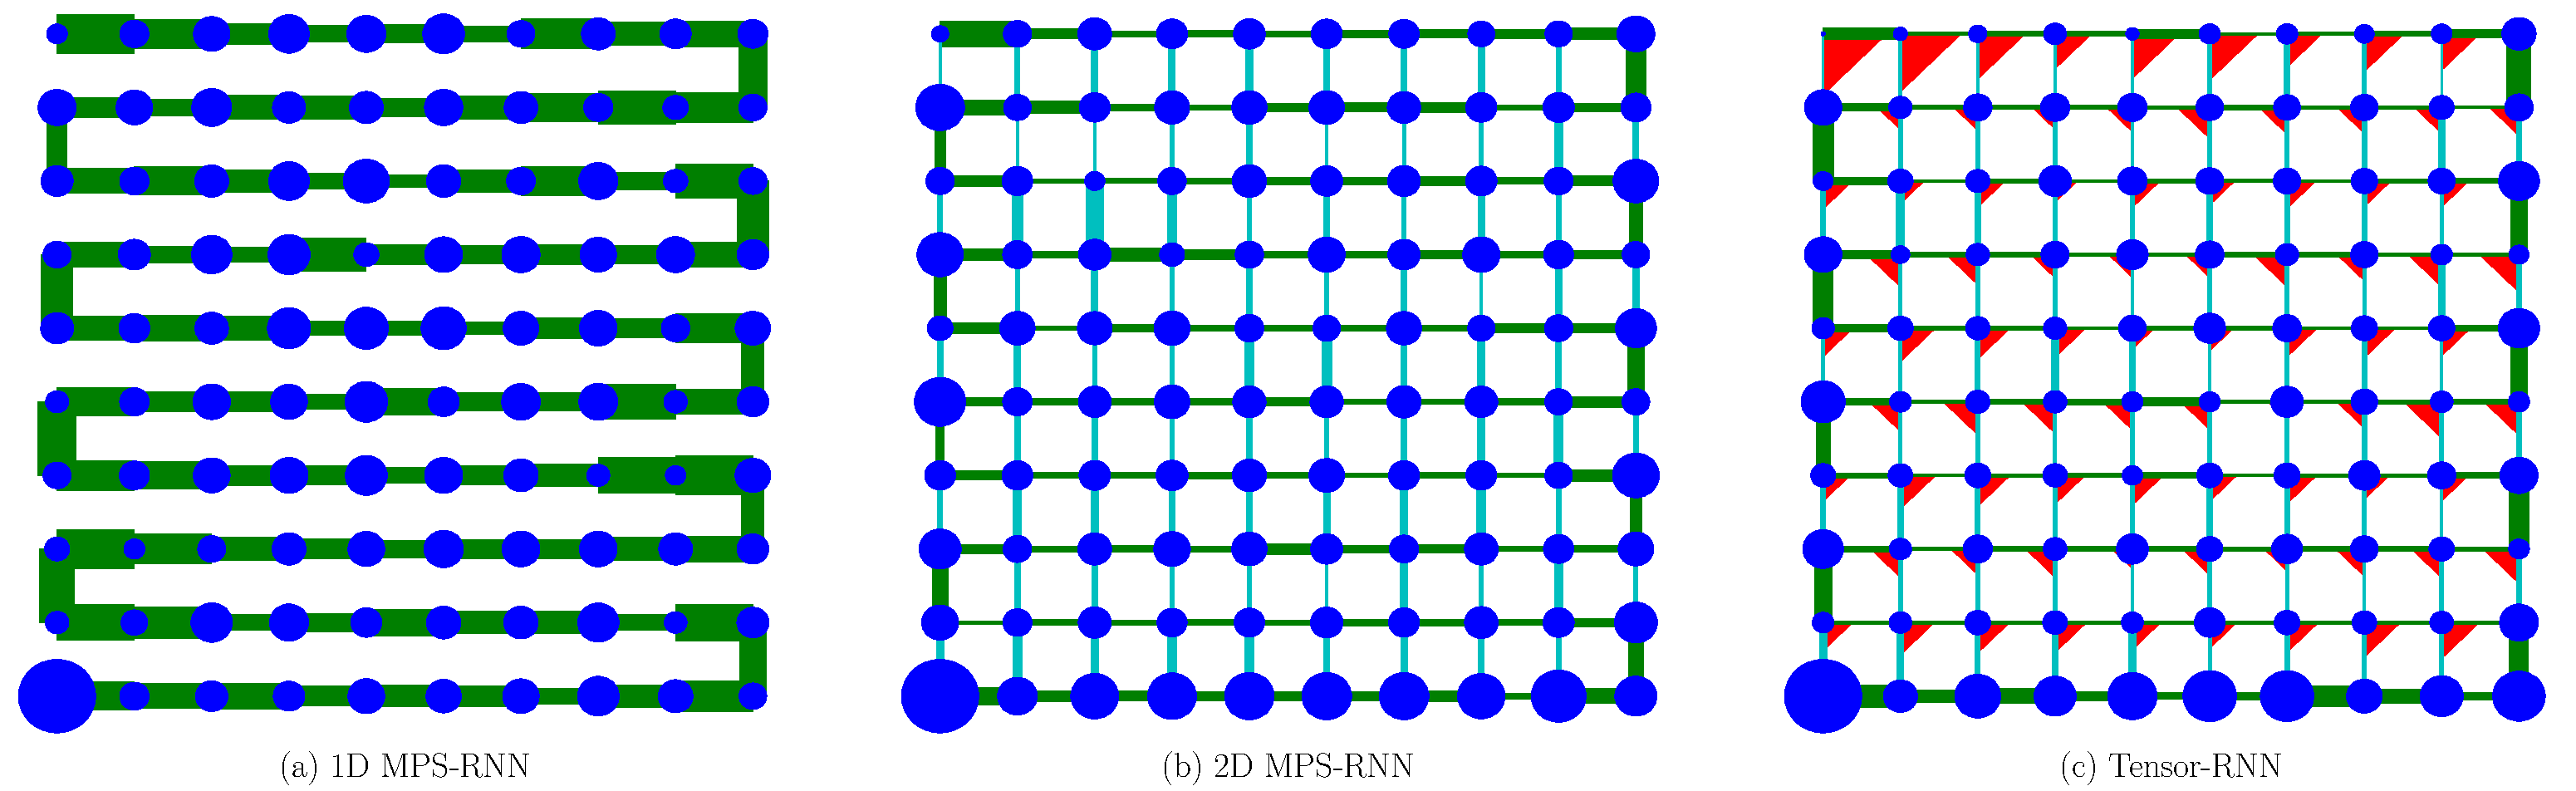
\includegraphics[width=\linewidth]{ch9/tensor_rnn_h_comp.pdf}
\caption[Magnitudes of tensor, matrix, and vector terms in tensor-RNN]{
This figure is reproduced from Fig.~S5 in the supplemental material of Ref.~\cite{wu2023tensor}.
}
\label{fig:tensor-rnn-h-comp}
\end{figure}

\chapter{VarBench: variational benchmarks for quantum many-body systems}
\label{ch:varbench}
